\documentclass[11pt]{beamer}
\usepackage[utf8]{inputenc}
\usepackage[T1]{fontenc}
\usepackage{lmodern}
\usepackage[spanish]{babel}
\usepackage{graphicx}
\usepackage[most]{tcolorbox}
\usetheme{Darmstadt}
\setbeamertemplate{navigation symbols}{}
\setbeamertemplate{footline}{
	\begin{beamercolorbox}[ht=3ex,leftskip=1.4cm,rightskip=.3cm]{author in head/foot}
		\hfill \insertframenumber
		\vspace*{0.07cm}
	\end{beamercolorbox}
}
\usepackage{url}
\usepackage{hyperref}
\usepackage{listings}

% color def
\usepackage{color}
\definecolor{darkred}{rgb}{0.6,0.0,0.0}
\definecolor{darkgreen}{rgb}{0,0.50,0}
\definecolor{lightblue}{rgb}{0.0,0.42,0.91}
\definecolor{orange}{rgb}{0.99,0.48,0.13}
\definecolor{grass}{rgb}{0.18,0.80,0.18}
\definecolor{pink}{rgb}{0.97,0.15,0.45}

\usepackage{nth}

% General Setting of listings
\lstset{
	language=Python,
	tabsize=4,
	aboveskip=1em,
	breaklines=true,
	abovecaptionskip=-6pt,
	captionpos=b,
	escapeinside={\%*}{*)},
	frame=single,
	numbers=left,
	numbersep=8pt,
	numberstyle=\tiny,
	morekeywords=[1]{,as,assert,nonlocal,with,yield,self,True,False,None,},
	morekeywords=[2]{,__init__,__add__,__mul__,__div__,__sub__,__call__,__getitem__,__setitem__,__eq__,__ne__,__nonzero__,__rmul__,__radd__,__repr__,__str__,__get__,__truediv__,__pow__,__name__,__future__,__all__,},
	morekeywords=[3]{,object,type,isinstance,copy,deepcopy,zip,enumerate,reversed,list,set,len,dict,tuple,range,xrange,append,execfile,real,imag,reduce,str,repr,},
	morekeywords=[4]{,Exception,NameError,IndexError,SyntaxError,TypeError,ValueError,OverflowError,ZeroDivisionError,},
	morekeywords=[5]{,ode,fsolve,sqrt,exp,sin,cos,arctan,arctan2,arccos,pi, array,norm,solve,dot,arange,isscalar,max,sum,flatten,shape,reshape,find,any,all,abs,plot,linspace,legend,quad,polyval,polyfit,hstack,concatenate,vstack,column_stack,empty,zeros,ones,rand,vander,grid,pcolor,eig,eigs,eigvals,svd,qr,tan,det,logspace,roll,min,mean,cumsum,cumprod,diff,vectorize,lstsq,cla,eye,xlabel,ylabel,squeeze,},
	deletekeywords=[2]{next,set},
	deletekeywords=[3]{next,set},
	basicstyle=\ttfamily\small,
	backgroundcolor=\color{white},
	commentstyle=\color{darkgreen}\slshape,
	keywordstyle=\color{blue}\bfseries\itshape,
	keywordstyle=[2]\color{blue}\bfseries,
	keywordstyle=[3]\color{grass},
	keywordstyle=[4]\color{red},
	keywordstyle=[5]\color{orange},
	stringstyle=\color{darkred},
	emphstyle=\color{pink}\underbar,
	morestring=*[d]{"},
    literate={á}{{\'a}}1 {é}{{\'e}}1 {í}{{\'i}}1 {ó}{{\'o}}1 {ú}{{\'u}}1 {ñ}{{\~n}}1 {Á}{{\'A}}1 {É}{{\'E}}1 {Í}{{\'I}}1 {Ó}{{\'O}}1 {Ú}{{\'U}}1 {Ñ}{{\~N}}1 {¿}{{\textquestiondown}}1 {¡}{{\textexclamdown}}1
}

\usepackage{tikz}
\usetikzlibrary{calc,shapes.multipart,chains,arrows,positioning}

\tikzset{
	squarecross/.style={
		draw, rectangle,minimum size=18pt, fill=orange!80,
		inner sep=0pt, text=black,
		path picture = {
			\draw[black]
			(path picture bounding box.north west) --
			(path picture bounding box.south east)
			(path picture bounding box.south west) --
			(path picture bounding box.north east);
		}
	},
	list/.style={
		very thick, rectangle split,
		rectangle split parts=2, draw,
		rectangle split horizontal, minimum size=18pt,
		inner sep=4pt, text=black,
		rectangle split part fill={red!20, blue!20}
	},
	->, start chain, very thick,
	chain_arrow/.style={*->, thick}
}


\begin{document}
	\author{Estructura de Datos}
	\title{Complejidad Algorítmica \\
	&
	\\
	Recursividad}
	\titlegraphic{
\includegraphics[width=3cm]{img/UPNA}}
	\date[]{2025-2026}
	\subject{Estructura de Datos}

	\begin{frame}[plain]
		\maketitle
	\end{frame}

	\begin{frame}
		\tableofcontents
	\end{frame}



\section{Midiendo la Complejidad}

	\subsection{¿Qué es la eficiencia?}

	\begin{frame}\frametitle{Eficiencia de los algoritmos}
	\begin{itemize}
	\item Varios métodos para implementar una solución a un problema
	\item ¿Cómo decidimos cuál es el mejor?
	\pause
	\item ¿El más fácil de entender?
	\pause
	\item ¿El que necesita menos tiempo?
	\pause
	\begin{itemize}
		\item ¿El algoritmo que requiere 1 segundo para analizar 10 datos requerirá 10 segundos para analizar 100?
	\end{itemize}
	\end{itemize}
	\end{frame}

	\subsection{Enfoque experimental}

	\begin{frame}[fragile]\frametitle{Usando el tiempo para medir la complejidad}
	\begin{lstlisting}
import time

def suma_menores_que(n):
    la_suma = 0
    for i in range(n):
        la_suma += i
    return la_suma

inicio = time.time()
suma_menores_que(10000000)
fin = time.time()
print(f"La suma necesitó {fin-inicio:.4} segundos")
# La suma necesitó 0.6202 segundos
\end{lstlisting}
	\end{frame}

	\begin{frame}[fragile]\frametitle{Se necesitan repeticiones}
	\begin{lstlisting}
# La suma necesitó 0.6202 segundos
# La suma necesitó 0.506 segundos
# La suma necesitó 0.468 segundos
# La suma necesitó 0.4748 segundos
# La suma necesitó 0.4771 segundos
# La suma necesitó 0.472 segundos
\end{lstlisting}
	\begin{block}{}
	\centering ¿Por qué disminuye el tiempo?
	\end{block}
	\pause
	\begin{itemize}
	\item Se necesitan mediciones repetidas y promediar los resultados
	\item Si modificamos \texttt{n}, ¿cómo cambiará el tiempo necesario?
	\end{itemize}
	\end{frame}

	\subsection{Enfoque formal}

	\begin{frame}\frametitle{Análisis matemático}
	\begin{itemize}
	\item Usar el tiempo necesario para ejecutar un algoritmo puede darnos una idea de su eficiencia
	\pause
	\item No es comparable 
	\begin{itemize}
		\item Qué lenguaje de programación se usa
		\item En qué ordenador se está ejecutando
	\end{itemize}
	\pause
	\item Se necesita un enfoque formal para definir la complejidad
	\begin{itemize}
		\item Complejidad temporal
		\item Complejidad espacial
	\end{itemize}
	\end{itemize}
	\end{frame}

	\begin{frame}[fragile]\frametitle{Contando operaciones}
	\begin{lstlisting}
def suma_menores_que(n):
    la_suma = 0				# 1 operación
    for i in range(n):
        la_suma += i		# n operaciones
    return la_suma
\end{lstlisting}
	\begin{itemize}
	\item El enfoque más básico es contar cuántas operaciones se necesitan para ejecutar el código
	\end{itemize}
	\pause
	\begin{block}{}
	\centering$T(n) = 1 + n$
	\end{block}
	\end{frame}


	\begin{frame}\frametitle{Notación Big O}
	\begin{itemize}
	\item Normalmente no nos interesa la expresión específica, solo una aproximación
	\item La notación Big O describe cómo crecerá un algoritmo
	\item $8n^2 + 13n + 1324 \Rightarrow O(n^2)$
	\end{itemize}
	\begin{center}
	\begin{tabular}{l|l}
	\hline
	\textbf{f(n)} & \textbf{Nombre} \\
	\hline
	1 &  Constante \\
	log n & Logarítmica \\
	n & Lineal \\
	n log n & Log-Lineal \\
	$n^2$ & Cuadrática \\
	$n^3$ & Cúbica \\
	$2^n$ & Exponencial \\
	\end{tabular}
	\end{center}
	\end{frame}

	\begin{frame}\frametitle{Gráfico Big O}
	\begin{figure}
	\centering
	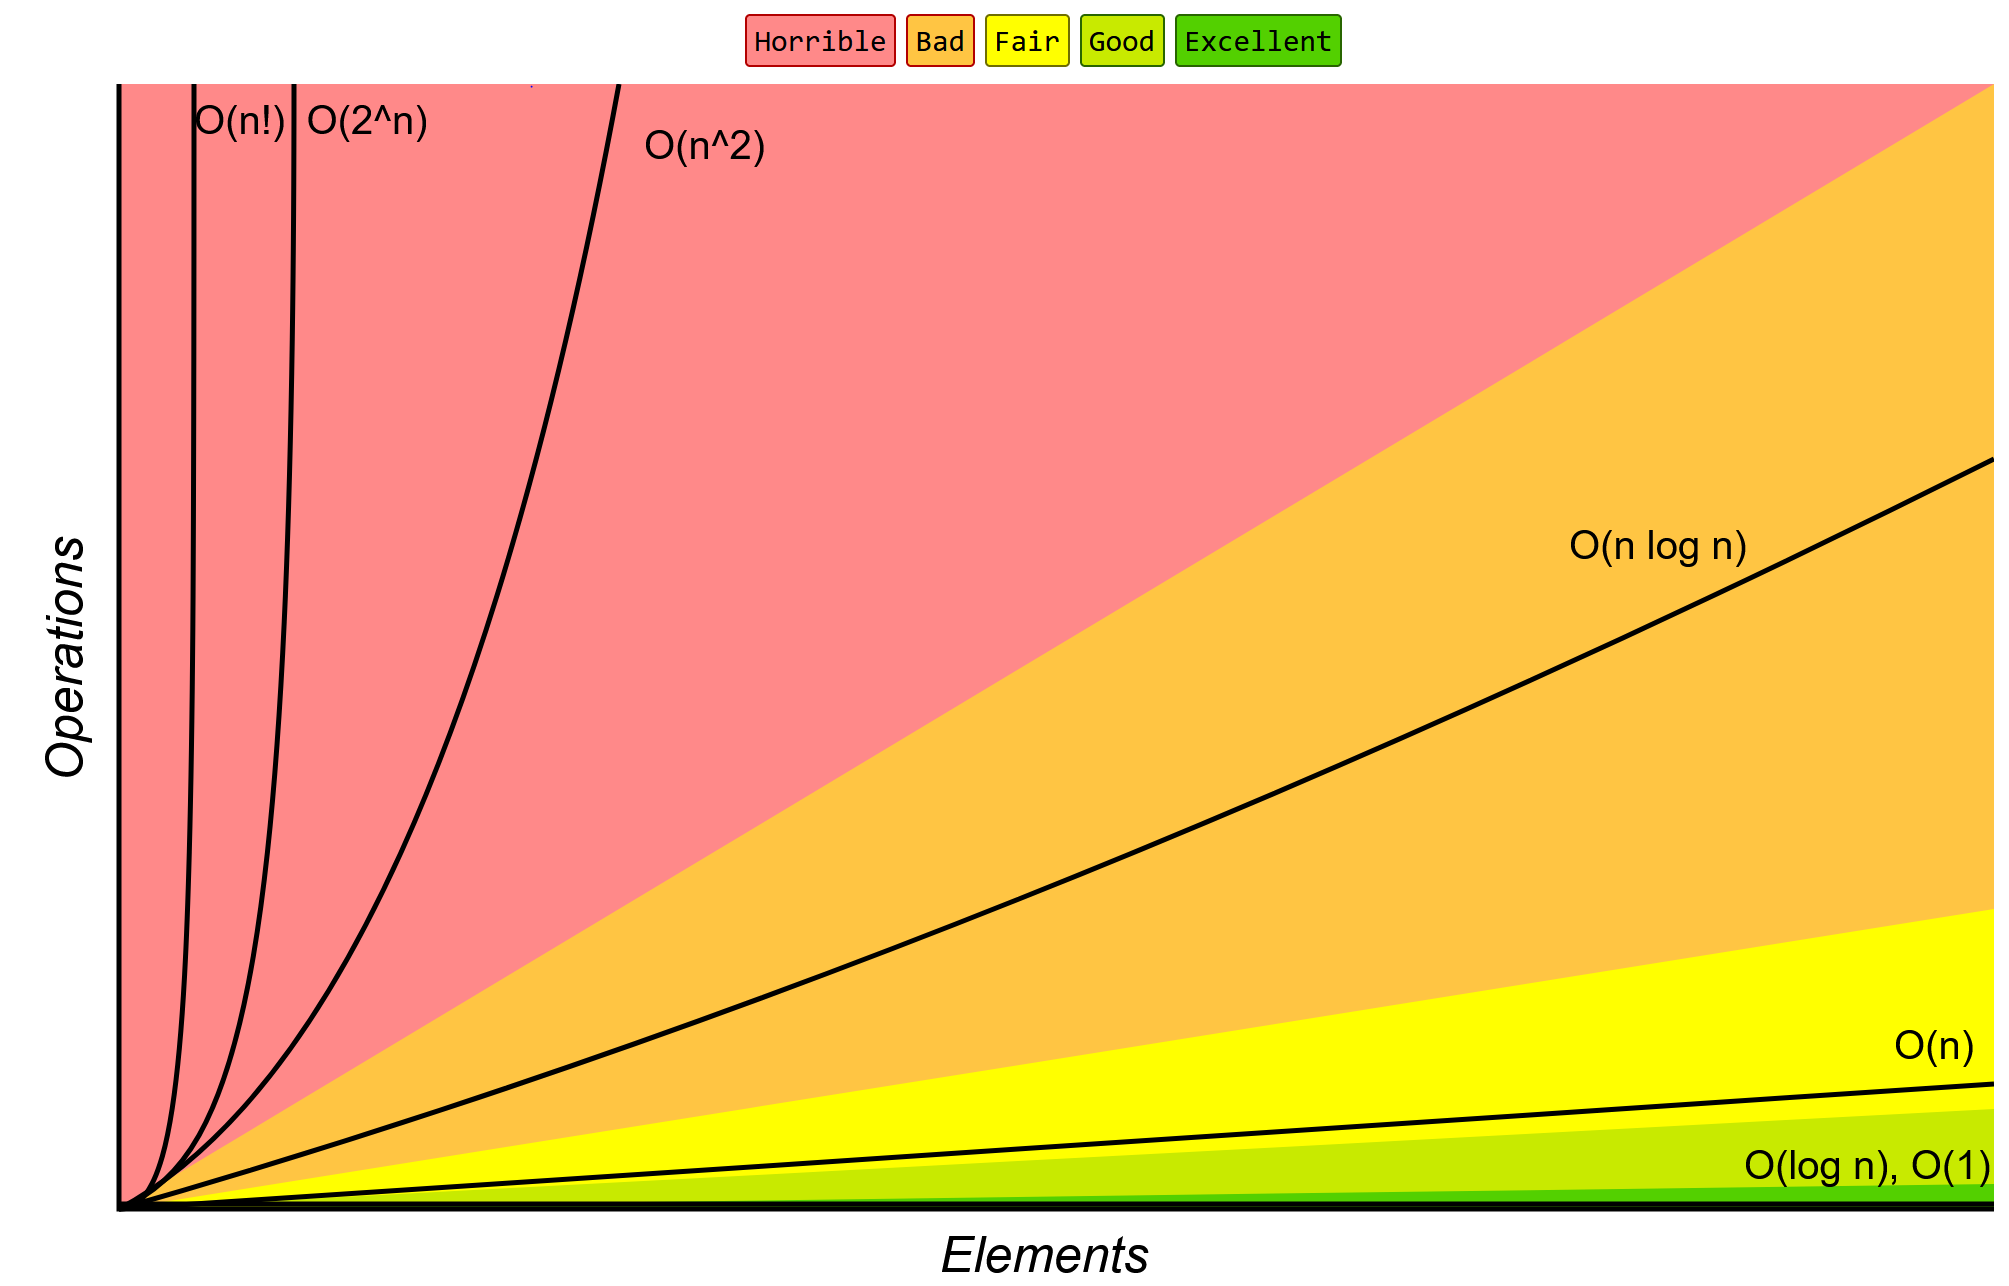
\includegraphics[width=0.9\linewidth]{img/bigo}
	\label{fig:bigo}
	\end{figure}
	\href{https://www.bigocheatsheet.com/}{https://www.bigocheatsheet.com/}
	\end{frame}

	\subsection{Ejercicios de complejidad}

	\begin{frame}[fragile, allowframebreaks]\frametitle{Ejemplo de complejidad}
	\begin{lstlisting}
n = 1000
b = 2
c = 3
for i in range(n):
	for j in range(n):
		x = i * i
		y = j * j
		z = i * j
for k in range(n):
	w = c * k + 15
	v = b * b
d = 33
\end{lstlisting}
	\framebreak
	\begin{lstlisting}
n = 1000				# 1
b = 2				# 1
c = 3				# 1
for i in range(n):
	for j in range(n):
		x = i * i		# n^2
		y = j * j		# n^2
		z = i * j		# n^2
for k in range(n):
	w = c * k + 15		# n
	v = b * b			# n
d = 33				# 1
\end{lstlisting}
	\begin{block}{}
	\centering$T(n) = 3 + 3n^2 + 2n + 1 \rightarrow O(n^2)$
	\end{block}
	\end{frame}

	\begin{frame}[fragile, allowframebreaks]\frametitle{Mínimo de una lista}
	\begin{block}{}
	Escribe una función que devuelva el valor mínimo en una lista de enteros. ¿Cuál es su complejidad?
	\end{block}
	\framebreak
	\begin{lstlisting}
def min_lista(lst):
	return min(lst) # ¿cuál es la complejidad de min()?
\end{lstlisting}
	\begin{block}{}
	\centering $O(?)$
	\end{block}
	\framebreak
	\begin{lstlisting}
def min_lista(lst):
	minimo = lst[0]		# 1
	for valor in lst:
		if valor < minimo:		# n
			minimo = valor		# menos de n
	return minimo
\end{lstlisting}
	\begin{block}{}
	\centering $O(n)$
	\end{block}
	\end{frame}

	\colorlet{lightgreen}{green!60!}

	\tcbset{on line, 
	        boxsep=4pt, left=0pt,right=0pt,top=0pt,bottom=0pt,
	        colframe=white,colback=lightgreen,  
	        highlight math style={enhanced}
	        }

	\begin{frame}[fragile]\frametitle{Ejercicio 1}
	\begin{lstlisting}
test = 0
for i in range(n):
	for j in range(n):
		test = test + i * j
\end{lstlisting}
	\begin{enumerate}
	\item $O(n)$
	\item \alt<2>{\tcbox{$O(n^2)$}}{$O(n^2)$}
	\item $O(log\ n)$
	\item $O(n^3)$
	\end{enumerate}
	\end{frame}

	\begin{frame}[fragile]\frametitle{Ejercicio 2}
	\begin{lstlisting}
test = 0
for i in range(n):
	test = test + 1
	
for j in range(n):
	test = test + 1
\end{lstlisting}
	\begin{enumerate}
	\item \alt<2>{\tcbox{$O(n)$}}{$O(n)$}
	\item $O(n^2)$
	\item $O(log\ n)$
	\item $O(n^3)$
	\end{enumerate}
	\end{frame}

	\begin{frame}[fragile]\frametitle{Ejercicio 3}
	\begin{lstlisting}
i = n
while i > 0:
	k = 2 + 2
	i = i // 2
\end{lstlisting}
	\begin{enumerate}
	\item $O(n)$
	\item $O(n^2)$
	\item  \alt<2>{\tcbox{$O(log\ n)$}}{$O(log\ n)$}
	\item $O(n^3)$
	\end{enumerate}
	\end{frame}

	\subsection{Complejidad de estructuras comunes}

	\begin{frame}\frametitle{Eficiencia de las listas de Python}
	\begin{center}
	\begin{tabular}{l|l}
	\hline
	\textbf{Operación} &\textbf{ Eficiencia Big O} \\
	\hline
	get & $O(1)$ \\
	set & $O(1)$ \\
	append & $O(1)$ \\
	insert(i, item) & $O(n)$ \\
	pop() & $O(1)$ \\
	pop(i) & $O(n)$ \\
	del & $O(n)$ \\
	contains & $O(n)$ \\
	reverse & $O(n)$ \\
	sort & $O(n\ log\ n)$ \\
	multiply & $O(nk)$ \\
	\end{tabular}
	\end{center}
	\end{frame}


	\begin{frame}\frametitle{Eficiencia de los diccionarios de Python}
	\begin{center}
	\begin{tabular}{l|l}
	\hline
	\textbf{Operación} &\textbf{ Eficiencia Big O} \\
	\hline
	get & $O(1)$ \\
	set & $O(1)$ \\
	del & $O(1)$ \\
	contains & $O(1)$ \\
	copy & $O(n)$ \\
	\end{tabular}
	\end{center}
	\end{frame}

	\section{Recursividad}

	\begin{frame}{Resumen}
	\tableofcontents[currentsection,hideothersubsections]
	\end{frame}

	\subsection{¿Qué es la recursividad?}
	\begin{frame}\frametitle{Recursividad}
	\begin{block}{}
	La recursividad es el proceso de repetir elementos de forma autosimilar
	\end{block}
	\begin{description}
	\item[Algorítmicamente:] una forma de diseñar soluciones a problemas mediante divide y vencerás o reduce y vencerás
	\begin{itemize}
		\item Reducir un problema a versiones más simples del mismo problema
	\end{itemize}
	\item[Semánticamente:] una técnica de programación donde una función se llama a sí misma
	\begin{itemize}
		\item Resolver el mismo problema sobre otra entrada con el objetivo de simplificar la entrada del problema mayor
	\end{itemize}
	\end{description}
	\end{frame}

	\begin{frame}\frametitle{Algoritmos iterativos VS recursivos}
	\begin{itemize}
	\item Las sentencias de bucle (bucles \texttt{while} y \texttt{for}) conducen a algoritmos iterativos
	\begin{itemize}
		\item Calculan usando un conjunto de variables de estado que se actualizan en cada iteración de los bucles
	\end{itemize}
	\item La recursividad es capaz de crear bucles sin necesidad de enfoques iterativos
	\end{itemize}
	\end{frame}

	\subsection{Recursividad mediante ejemplos}

	\begin{frame}[fragile]\frametitle{Multiplicación - Iterativa}
	\begin{block}{}
	\centering $a \times b$ es equivalente a sumar a a sí mismo b veces
	\end{block}
	\begin{lstlisting}
def multiplica_iter(a, b):
	resultado = 0
	for i in range(b):
		resultado += a
	return resultado
\end{lstlisting}
	\end{frame}

	\begin{frame}[fragile]\frametitle{Multiplicación - Recursiva}
	\begin{block}{Reducir el problema a uno más pequeño}
	\centering $a \times b$ es equivalente a $a + (a  \times (b - 1))$
	\end{block}
	\begin{block}{Caso base}
	\centering cuando $b = 1$ entonces $a \times b = a$
	\end{block}
	\pause
	\begin{lstlisting}
def multiplica_recur(a, b):
	if b == 1:
		return a
	else:
		return a + multiplica_recur(a, b - 1)
\end{lstlisting}
	\end{frame}

	\begin{frame}[fragile]\frametitle{Factorial}
	\begin{block}{}
	\centering $n! = n \times (n - 1) \times (n - 2) \times (n - 3) \times \ldots \times 1$
	\end{block}
	\begin{description}
	\item[Caso base:] Sabemos que el factorial de 1 es 1
	\item[Reducir el problema:] El factorial de n es $n \times (n - 1)!$
	\end{description}
	\pause
	\begin{lstlisting}
def fact(n):
	if n == 1:
		return n
	else:
		return n * fact(n-1)
\end{lstlisting}
	\end{frame}

	\subsection{Reglas}

	\begin{frame}\frametitle{Características de la recursividad}
	\begin{itemize}
	\item En algunos casos la recursividad puede ser más simple e intuitiva
	\item La recursividad puede ser eficiente desde el punto de vista del programador
	\item La recursividad puede no ser eficiente desde el punto de vista del ordenador
	\begin{block}{}
	La recursividad necesita crear una pila de llamadas (call stack) para las llamadas recursivas, y mantener esas variables en memoria. Es fácil crear un algoritmo que no sea eficiente.
	\end{block}
	\end{itemize}
	\end{frame}

	\begin{frame}\frametitle{Resumen}
	\begin{itemize}
	\item Todos los algoritmos recursivos tienen un caso base
	\item Todos los algoritmos recursivos deben cambiar su estado (en cada recursión) y acercarse al caso base
	\item Un algoritmo recursivo es un algoritmo que se llama a sí mismo
	\end{itemize}
	\end{frame}

	\subsection{Ejercicios}

	\begin{frame}\frametitle{Sumar elementos de una lista}
	\begin{block}{Crea un algoritmo recursivo que devuelva la suma de todos los elementos de una lista}
No uses la función \texttt{sum()}
\end{block}
	\begin{block}{¿Cuántas llamadas son necesarias para calcular la suma de las siguientes listas?}
\texttt{[3, 4, 6, 8, 0, 10, 11]} \\
\texttt{['3']} \\
\texttt{[]}
\end{block}
	\end{frame}


	\begin{frame}[fragile]\frametitle{Sumar elementos de una lista: solución}
	\begin{lstlisting}
def suma_lista(lst):
    if len(lst) == 1:
        return lst.pop()
    else:
        return lst.pop() + suma_lista(lst)
\end{lstlisting}
	\end{frame}

	\begin{frame}\frametitle{La sucesión de Fibonacci}
	\begin{itemize}
	\item La sucesión de Fibonacci se define por las siguientes ecuaciones:
	\begin{equation*}
	\begin{aligned}
	f_0 &= 0\\
f_1 &= 1\\
f_n &= f_{n-1} + f_{n-2}
	\end{aligned}
	\end{equation*}
	\item Implementa un algoritmo recursivo para obtener cualquier número de la sucesión de Fibonacci
	\end{itemize}
	\end{frame}

	\begin{frame}[fragile]\frametitle{La sucesión de Fibonacci: solución}
	\begin{lstlisting}
def fibonacci(n):
	if n == 0:
		return 0
	elif n == 1:
		return 1
	else:
		return fibonacci(n-1) + fibonacci(n-2)
\end{lstlisting}
	\begin{block}{Eficiencia}
La solución mostrada aquí es highly ineficiente, intenta calcular el número de Fibonacci \nth{10}, \nth{20} y \nth{30}, ¿aumentó el tiempo de forma lineal?\¿Cómo podemos mejorarlo?
	\end{block}
	\end{frame}

	\begin{frame}\frametitle{Invertir una lista in situ}
	\begin{block}{Crea una función que sea capaz de invertir una lista de manera recursiva}
La lista debe invertirse in situ. Esto significa que no se pueden crear listas y no se permite el troceado (slicing) de listas.
\end{block}
	\begin{description}
	\item[Un pequeño consejo:] La función que crees no tomará solo la lista, sino también los índices de inicio y fin para intercambiar. En cada iteración intercambia los valores de los índices de inicio y fin y modifícalos en consecuencia.
	\end{description}
	\end{frame}

	\end{document}